\documentclass[final]{beamer}
%% Possible paper sizes: a0, a0b, a1, a2, a3, a4.
%% Possible orientations: portrait, landscape
%% Font sizes can be changed using the scale option.
\usepackage[size=a0,orientation=portrait,scale=1.1]{beamerposter}

\usetheme{gemini}
\usecolortheme{seagull}
\useinnertheme{rectangles}

% ====================
% Packages
% ====================

\usepackage[utf8]{inputenc}
\usepackage{graphicx}
\usepackage{booktabs}
\usepackage{tikz}
\usepackage{pgfplots}

% ====================
% Lengths
% ====================

% If you have N columns, choose \sepwidth and \colwidth such that
% (N+1)*\sepwidth + N*\colwidth = \paperwidth
\newlength{\sepwidth}
\newlength{\colwidth}
\setlength{\sepwidth}{0.03\paperwidth}
\setlength{\colwidth}{0.45\paperwidth}

\newcommand{\separatorcolumn}{\begin{column}{\sepwidth}\end{column}}
\newcommand{\blankfigure}[3]{
	\begin{figure}
		\centering
		\begin{tikzpicture}
			\draw[gray, line width=1.2pt] (0,0) rectangle (#1,#2);
		\end{tikzpicture}
		\caption{#3}
	\end{figure}
}

% ====================
% Logo (optional)
% ====================

\logoleft{
	\hspace{5cm}
\includegraphics[height=10 cm]{logos/nycu.png}
}
\logoright{
	
\includegraphics[height=10 cm]{logos/nycu.png}\hspace{5cm}
}

% ====================
% Footer (optional)
% ====================

\footercontent{
	2026 Deep Learning Final Project Presentation \hfill
	\insertdate \hfill
	BEHAVIOR-1K VLA Action Chunk Correction
}

% ====================
% My own customization
% - BibLaTeX
% - Boxes with tcolorbox
% - User-defined commands
% ====================
\input{custom-defs.tex}

%% Reference Sources
\addbibresource{refs.bib}
\renewcommand{\pgfuseimage}[1]{\includegraphics[scale=2.0]{#1}}

\title{Residual Action Chunk Correction for OpenPI-Comet on BEHAVIOR-1K}

\author{LIN, JIN-CHENG \and LIN, TING-WEI \and CHU, YI-TING}

\institute[shortinst]{Deep Learning Final Project}

\date{June 2026}

\begin{document}
	
\begin{frame}[t]
	
	\vspace*{-2ex}

	\begin{columns}[t]
	
	\begin{column}{2\colwidth+\sepwidth}
	\begin{block}{Project Overview}
		
		We study whether an Asynchronous Action Chunk Correction (A2C2) module can
		improve a frozen OpenPI-Comet VLA policy on BEHAVIOR-1K without retraining
		the base model.
		
		OpenPI-Comet predicts 32-step action chunks. At execution offset $k$, A2C2
		uses the latest observation to predict a 23-D residual:
		$$
		a^{exec}_{t+k} = a^b_{t,k} + \lambda \Delta a_{t,k}.
		$$

		
	\end{block}
	\end{column}

	\end{columns}

	\begin{columns}[t]
		\separatorcolumn
		
		\begin{column}{\colwidth}
			
			\begin{exampleblock}{Task Selection}
				
				We first reproduced OpenPI-Comet fixed-seed rollouts and used the local
				$q_{final}$ statistics to select representative tasks for setup validation.
				Task 18 is kept as the main correction target because it shows partial but
				non-saturated baseline progress.
				
				\begin{table}
					\centering
					\begin{tabular}{l l c c c c c c}
						\toprule
						\textbf{ID} & \textbf{Task} & \textbf{Mean} & \textbf{Median} &
						\textbf{Min} & \textbf{Max} & \textbf{$>0$} & \textbf{Avg Frames} \\
						\midrule
						1 & Picking Up Trash & 0.8333 & 1.0000 & 0.3333 & 1.0000 & 100\% & 5268 \\
						7 & Picking Up Toys & 0.1833 & 0.0833 & 0.0000 & 0.6667 & 50\% & 18891 \\
						18 & Tidying Bedroom & 0.1333 & 0.0000 & 0.0000 & 0.6667 & 30\% & 11037 \\
						\bottomrule
					\end{tabular}
					\caption{Local OpenPI-Comet fixed-seed rollout statistics for selected tasks.}
				\end{table}
				
			\end{exampleblock}
	
			
			\begin{block}{Correction Head Inputs}
				
				The implemented A2C2 head is a multimodal token-fusion model rather than a
				state-only MLP.
				
				\begin{itemize}
					\item \textbf{Source-frame context:} cached action chunk, selected action,
					valid mask, OpenPI-Comet prefix latent $z_t$, and inference timing.
					\item \textbf{Execution-frame context:} proprioception, RGB observations,
					task language, camera-relative pose, and task-info features.
					\item \textbf{Model structure:} token projections, language GRU, frozen
					ResNet-18 visual encoders, six-layer Transformer encoder, and residual MLP.
				\end{itemize}
				
				\begin{figure}
					\centering
					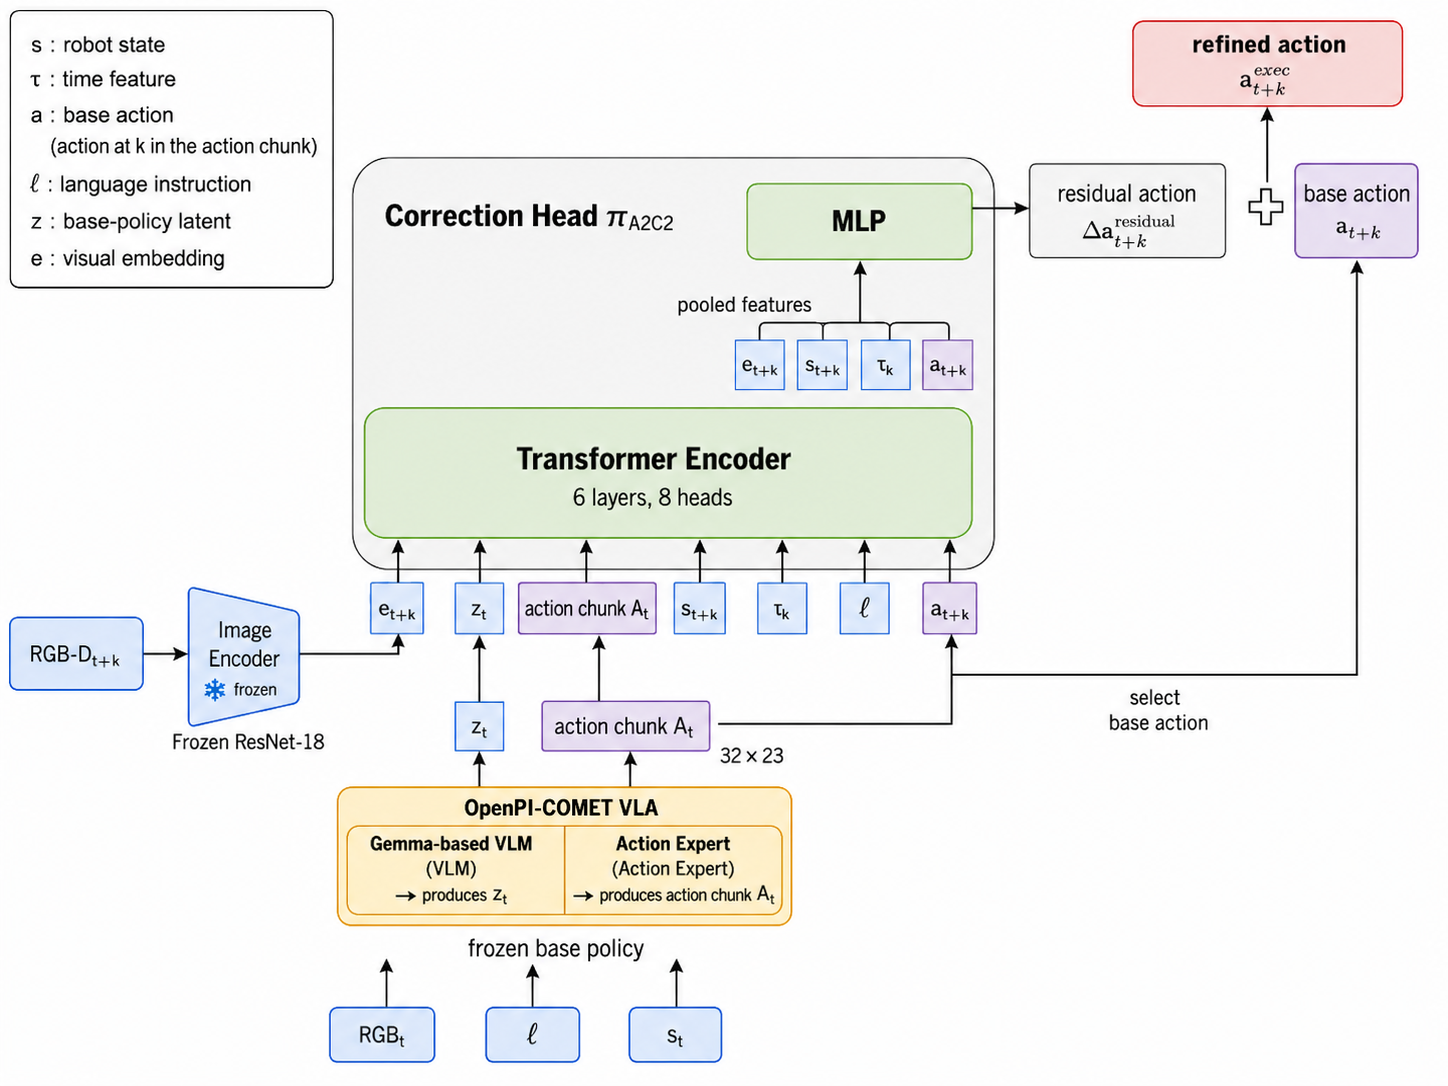
\includegraphics[height=28cm]{image/a2c2_architecture.png}
					\caption{A2C2 correction-head architecture and residual action composition.}
				\end{figure}
				
			\end{block}

			\begin{alertblock}{Why Did A2C2 Hurt Performance?}
				
				Even though the validation corrected MSE is roughly half of the base action MSE, 
				the evaluation performance still dropped significantly.
				Our diagnosis is that the current objective treats
				a heterogeneous, bounded robot action vector as a homogeneous residual
				regression problem:
				$$
				L = \|\Delta a_{pred} - (a_{expert} - a^b_{t,k})\|_2^2.
				$$
				
				\begin{itemize}
					\item \textbf{Scale mismatch:} arm/torso dimensions can dominate the loss,
					while small-range gripper errors remain weakly supervised.
					\item \textbf{Behavior mismatch:} gripper commands are event-like; MSE can
					average open/close actions into invalid half-open behavior.
					\item \textbf{Policy mismatch:} a large residual can perturb a coherent
					action chunk generated by the frozen flow policy.
				\end{itemize}
				
			\end{alertblock}

			\begin{defbox}{Range-Normalized Residual Loss}

				We keep the residual target unchanged:
				$$
				\Delta a^*_{t,k} = a^*_{t+k} - a^b_{t,k}.
				$$
				For each action dimension $j$, we estimate a robust scale from the training
				split and normalize residual errors:
				$$
				s_j = \max\left(Q_{0.99}(a_j)-Q_{0.01}(a_j), \epsilon\right),
				\quad
				e_j = \frac{\hat{\Delta a}_j - \Delta a^*_j}{s_j}.
				$$
				Then we aggregate errors by action group:
				$$
				L_{\text{group}} =
				\sum_{g \in \mathcal{G}} w_g
				\frac{1}{|g|}\sum_{j \in g} \rho(e_j),
				$$
				where $\mathcal{G}$ contains base, torso, left/right arm, and left/right
				gripper groups. We compare normalized MSE, normalized Huber, and a
				gripper-weighted Huber variant with $w_g=2.0$ for grippers and $w_g=1.0$
				otherwise. This directly tests whether the failure comes from scale
				imbalance, outlier residuals, or weak gripper supervision.

			\end{defbox}
			
		\end{column}
	
		\separatorcolumn
		
		\begin{column}{\colwidth}
			
			\begin{exampleblock}{Results}{}

				We evaluate Task 1 (Picking Up Trash) with fixed-seed online rollouts over
				ten instances.  The ablation compares the frozen OpenPI-Comet baseline
				against A2C2 residual-correction variants trained for 200k steps:
				(i) raw MSE, (ii) normalized MSE, (iii) normalized Huber (iv) the full setting with
				normalization, Huber loss, and gripper weighting. All the validation corrected mse are smaller than base action mse. 
		
				\begin{table}
						\centering
						\begin{tabular}{l l r r c}
								\toprule
								\textbf{Policy} & \textbf{Ablation} & \textbf{Mean $q_{final}$} & \textbf{SD} & \textbf{Nonzero IDs} \\
								\midrule
								Comet & Frozen baseline & 0.8333 & 0.2236 & \\
								Comet + A2C2 & MSE &  &  &  \\
								Comet + A2C2 & Norm-MSE &  &  &  \\
								Comet + A2C2 & Norm-Huber &  &  &  \\
								Comet + A2C2 & All (Norm + Huber + GripW) & 0.1000 & 0.2134 & 2/10 \\
								\bottomrule
						\end{tabular}
						\caption{Task 1 fixed-seed online evaluation over ten instances.}
				\end{table}
		
		  \end{exampleblock}

			\begin{thm}{Potential Risk: Random Chunk Supervision Can Break Mode Consistency}{}
				
				The base flow policy samples a temporally coherent action chunk:
				$$
				A^b_t \sim \pi_b(A_t \mid o_t, \ell).
				$$
				However, A2C2 is trained with randomly sampled chunk offsets. For an offset
				$k$, the residual target is defined locally as
				$$
				\Delta a^{target}_{t,k}
				=
				a^{expert}_{t+k} - a^b_{t,k}.
				$$

				This provides only local one-step supervision. If multiple valid chunks exist
				under similar observations, the sampled expert action may belong to a different
				mode from the base action chunk. Then the residual head is trained to partially
				pull a coherent base chunk toward a locally different expert mode:
				$$
				a^b_{t,k} + \Delta a_\phi
				\approx
				a^{expert}_{t+k}.
				$$

				As a result, the correction may not collapse an entire trajectory, but it can
				break chunk-level mode consistency. The corrected action sequence may mix
				parts of different modes, reducing the temporal coherence originally produced
				by the flow-based base policy.
				
			\end{thm}
			
			\begin{block}{Discussion}
				
				The result is negative but informative. The implementation matches the A2C2
				formulation: it keeps OpenPI-Comet frozen, trains expert-minus-base
				residuals, uses latest execution-frame RGB/proprioception/language, and
				deploys the head inside an online receding-horizon control loop.
				
				\begin{itemize}
					\item \textbf{Offline-online mismatch:} training states come from expert
					demonstrations, but online rollouts visit policy-induced states with missed
					grasps, contact errors, and shifted object poses.
					\item \textbf{Action-scale imbalance:} raw MSE may be dominated by large arm
					coordinates while small gripper/contact dimensions remain task-critical.
					\item \textbf{Overcorrection:} an unconservative residual can perturb a base
					policy that was already partially competent.
				\end{itemize}
				
				\blankfigure{13}{3}{To be edited.}
				
			\end{block}
			
			\begin{block}{Conclusion and Next Steps}
				A2C2 does not improve Task 18 under the current configuration, reducing mean
				$q_{final}$ from 0.1333 to 0.0000. The next iteration should focus on making
				the residual module more conservative and better matched to online states.
				
				\begin{itemize}
					\item Normalize or reweight the loss by action dimension.
					\item Ablate correction scales such as 0.25, 0.5, and 1.0.
					\item Add residual norm clipping and an uncertainty gate that can keep the
					base action unchanged.
					\item Analyze performance by chunk offset to separate stale-chunk errors from
					missing high-level capability.
					\item Add online data, rollout-state relabeling, or hard-negative states.
				\end{itemize}
			\end{block}
		\end{column}
		
		\separatorcolumn
	\end{columns}
\end{frame}
\end{document}
